\documentclass[mathserif, aspectratio=169]{beamer}
%
%%%%%%%%%%%%%%%%%%%%%%%%%%%%%%%%%%%%%%%%%%%%%%%%%%%%%%%%%%%%%%%%%%%%%%%%
% need to split the includes to make spell checking work.
\usepackage{arev, arevmath}
\usepackage[scaled]{cabin}
\usepackage[T1]{fontenc}
\usepackage[super]{nth}
\usepackage{pifont}
\usepackage{wasysym}
\usepackage{tabularx}
\usepackage{array}
\usepackage{booktabs}
\usepackage{boldline}
\usepackage{colortbl}
%\usepackage{amsmath}
\usepackage{bm}
\usepackage{tcolorbox}
\usepackage{adjustbox}
\usepackage{minibox}
\usepackage{makecell}
\usepackage{adjustbox}
\usepackage{textcomp}
\usepackage[absolute,overlay]{textpos}
\setlength{\TPHorizModule}{1mm}%
\setlength{\TPVertModule}{1mm}%
\tcbuselibrary{skins}

\makeatletter
\newcommand{\antsize}{\@setfontsize{\antsize}{4pt}{4pt}}
\makeatother
\newcommand{\at}{\makeatletter @\makeatother}

\newcommand{\cmark}{\ding{51}}%
\newcommand{\bottomline}[1]{\vskip0pt plus 1fill{\alert{#1}\phantom{g}\vskip 1.0mm}}

\newcommand{\Quote}[2]{%
	\begin{center} 
		\begin{minipage}{0.7\textwidth} 
			\hrule
			\vskip 3mm
			\emph{{\color{ICTPblue} ``#1''}
			
			~~~~ {\color{ICTPorange} --- #2}}
			\vskip 3mm
			\hrule
			\vskip 2mm
		\end{minipage}
	\end{center}}


\mode<presentation>%
{
	\usetheme{default}
	%\usetheme[width=2.5cm]{PaloAlto}
	\usecolortheme{dove}
	\useoutertheme{infolines}
	% oder auch nicht

	% ICTP Colors
	\definecolor{ICTPblue}{RGB}{37,86,162} % 0x255682
	\definecolor{ICTPorange}{RGB}{255,130,0} % 0xff8200
	\definecolor{ICTPgreen}{RGB}{0,100,0}
	\definecolor{ICTPdark}{RGB}{80,80,80} % 0x505050
	\definecolor{ICTPlight}{RGB}{120,120,120}
	\definecolor{ICTPbrown}{RGB}{178,91,0}

	\definecolor{codebg}{rgb}{0.95,0.95,0.95}

	% Color theme
	\setbeamercolor{alerted text}{fg=ICTPorange}
	\setbeamercolor{frametitle}{fg=ICTPblue}
	\setbeamercolor{title}{fg=ICTPblue}
	\setbeamercolor{subtitle}{fg=ICTPorange}
	\setbeamercolor{normal text}{fg=ICTPdark}
	\setbeamercolor{author in foot}{fg=ICTPblue}
	\setbeamercolor{item}{fg=ICTPblue}
	\setbeamercolor{footline}{fg=ICTPblue}
	%\setbeamercolor{item projected}{bg=ICTPorange}
	%\setbeamercolor{item projected}{fg=white}

	\setbeamertemplate{headline}
	{}
	\setbeamertemplate{frametitle}
	{
		%\textbf{{\insertframetitle\phantom{g}}}\\
		%\textbf{\insertframetitle\phantom{g}}\\
		\textbf{\underline{\insertframetitle\phantom{g}}}\\
		%\textbf{\underline{\insertframetitle}}\\
		\vskip 1.0mm
		%{\color{UOLgold}\hrule height 2pt}
		%\par
	}
	\addtobeamertemplate{frametitle}{}{\vspace{-1em}}
	\setbeamertemplate{footline}{
		{%
			\textbf{ \hskip 3.0mm\insertshorttitle\phantom{.}---\phantom{.}\insertshortinstitute\hfill\insertframenumber\,/\,\inserttotalframenumber\hskip 3.0mm} 
		}
	}

	\setbeamertemplate{navigation symbols}{}%remove navigation symbols
	\setbeamertemplate{itemize items}[circle]
	\setbeamertemplate{enumerate items}[fg=ICTPblue]
	\setbeamercolor{itemize items}{fg=ICTPblue}
	\setbeamercolor{sidebar}{bg=ICTPblue}
	\setbeamercolor{title in sidebar}{fg=ICTPorange}
	\setbeamercolor{author in sidebar}{fg=ICTPorange}
	\setbeamercolor{section in sidebar}{fg=ICTPorange}
}

%\input{tikz/common-styles}

\usepackage{graphicx}
\usepackage[latin1]{inputenc}

\graphicspath{{../figs/}{../figs/common/}{../figs/islr/}}

\title[Statistical Learning] % (optional, nur bei langen Titeln n�tig)
{\textbf{Introduction to Statistical Learning\\ {\it with applications in Python}}\\%
		\href{www.statlearning.com}%
		{\tiny\it Based on ``Introduction to Statistical Learning, with applications in R'' by Gareth James, Daniela Witten, Trevor Hastie, Robert Tibishirani}\vspace{2em}}
		\vspace{-2.5cm}{}


		\author{\href{mailto:?to=Kurt Rinnert <kurt.rinnert@cern.ch>&subject=PWF Statistical Learning}{Kurt Rinnert}}

\institute[{\href{https://www.ictp.it/physics-without-frontiers.aspx}{Physics Without Frontiers} --- \href{https://www.ictp.it/}{ICTP}}] % (optional)
{\color{ICTPblue}\bfseries \href{https://www.ictp.it/physics-without-frontiers.aspx}{Physics Without Frontiers}\\\vspace{1mm}%
\href{https://www.ictp.it/}{
\includegraphics[width=0.20\textwidth]{common/ICTP-logo-full-trans.png}}\\%
\href{https://www.liverpool.ac.uk/physics/}{
\includegraphics[width=0.2\textwidth]{common/uol_logo.png}}}

\date{}

\titlegraphic{
	\texorpdfstring{\vspace{-2.8cm}}{}
	 \begin{minipage}[b][1.3cm][b]{0.26\textwidth}\color{ICTPlight}\antsize
		Copyright \textcopyright~2019\\
		\href{mailto:?to=Kurt Rinnert <kurt.rinnert@cern.ch>&subject=PWF Statistical Learning}{Kurt Rinnert <kurt.rinnert{\tt @}cern.ch>},
		\href{mailto:?to=Kate Shaw <kshaw@ictp.it>&subject=PWF Statistical Learning}{Kate Shaw <kshaw{\tt @}ictp.it>}\\
		Copying and distribution of this file, with or without modification,
		are permitted in any medium without royalty provided the copyright
		notice and this notice are preserved.  This file is offered as-is,
		without any warranty.


		Some of the figures in this presentation are taken from ``An Introduction to
		Statistical Learning, with applications in R''  (Springer, 2013) with
		permission from the authors: G. James, D. Witten,  T. Hastie and R. Tibshirani 
	 \end{minipage}\hspace{10cm}
}


\addtocounter{framenumber}{-1}

% nicer table row separation
\renewcommand{\arraystretch}{1.2}

% color boxes
\newcommand{\tabboxset}{\tcbset{enhanced, nobeforeafter, boxrule=0pt, boxsep=0pt, colback=codebg, colframe=codebg, coltext=ICTPdark, rounded corners, arc=4pt, fonttitle={\bfseries\tiny}}}
\newcommand{\codeboxset}{\tcbset{enhanced, nobeforeafter, boxrule=0pt, boxsep=0pt, colback=codebg, colframe=codebg, coltext=ICTPdark, rounded corners, arc=4pt, fonttitle={\bfseries\tiny}}}

\newcommand{\orange}{\color{ICTPorange}}
\newcommand{\blue}{\color{ICTPblue}}
\newcommand{\dark}{\color{ICTPdark}}
\newcommand{\R}{\mathbb{R}}
\newcommand{\dat}[1]{{\footnotesize\tt\orange #1}}
\newcommand{\e}[1]{\emph{#1}}
\newcommand{\bh}{\hat{\beta}}
\newcommand{\h}{\hat}

\makeatletter
\newcommand{\includegraphicsdpi}[3]{%
	\pdfimageresolution=#1%
	\includegraphics[#2]{#3}%
	\pdfimageresolution=72%
}

\newenvironment{blurb}%
	{\begin{center}\begin{minipage}{0.6\textwidth}\footnotesize}
	{\end{minipage}\end{center}}

\newenvironment{cpage}%
	{\begin{center}\begin{minipage}{0.75\textwidth}}
	{\end{minipage}\end{center}}

\newenvironment{popblock}[2]%
	{\begin{center}\begin{minipage}{#1}\footnotesize
		\begin{tcolorbox}[colframe=codebg, colback=white, colupper=ICTPdark, title={\normalsize\bfseries\blue #2}]}
	{\end{tcolorbox}\end{minipage}\end{center}}
\makeatother

\subtitle{\bfseries%
  {Resampling Methods}\\%
  {\tiny\it Cross-Validation for Regression, Validation Set, Leave-One-Out, $k$-Fold, Cross-Validation for Classification, Bootstrap}\\%
}
\begin{document}
\frame[plain]{
	\vskip 1.0mm
	\titlepage
	\vskip 1.0mm
}


\begin{frame}{Abstract}
	\begin{blurb}
		We already mentioned the importance of evaluating models on test data sets that
		were not used in the training phase. We now expand on this idea.

		Resampling methods are based on the idea of repeatedly drawing samples from a training
		data set and refitting the model in order to better evaluate the fitted model.

		These methods used to be computationally prohibitive because they involve multiple
		model fits. This is no longer a problem due to cheaply available computing resources.
	\end{blurb}
\end{frame}

\begin{frame}{Overview}
	\begin{itemize}
		\item Cross-Validation
		\item The Validation Set Approach 
		\item Leave-One-Out Cross-Validation (LOOCV)
		\item $k$-Fold Cross-Validation
		\item Cross-Validation for Classification
		\item The Bootstrap Method
	\end{itemize}
	\bottomline{All these methods provide \e{estimates} of the test error.}
\end{frame}

\begin{frame}{Cross-Validation}
	\begin{itemize}
		\item We have already discussed the difference between \e{training error rate} 
			and the \e{test error rate.}
		\item We can easily calculate the test error if we have a sufficiently large 
			test data set.
		\item In the absence of a dedicated test data set we can use a subset of the
			training data to estimate the test error.
		\item This subset is called the \e{validation set} or \e{hold-out set}.
	\end{itemize}
	\bl{We first assume regression and deal with classification later.}
\end{frame}

\begin{frame}{The Validation Set Approach}
	\begin{center}
		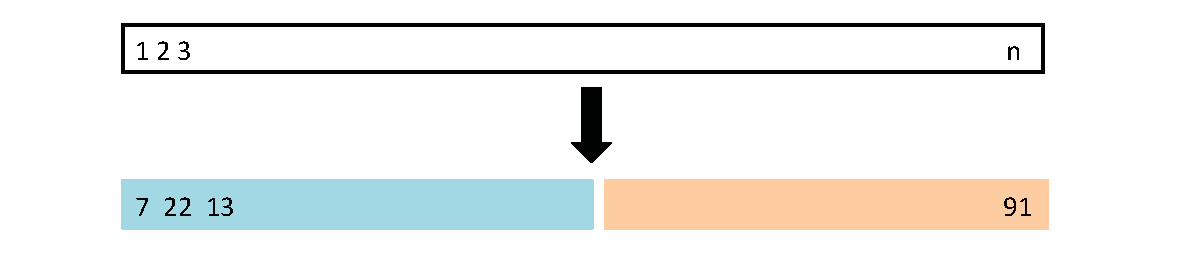
\includegraphics[width=0.8\textwidth]{5_1}
	\end{center}
	\begin{itemize}
		\item We \e{randomly} split the training data into a training set and
			a validation set.
		\item The model is then fit on the training set and evaluated on the
			validation set.
		\item In case of a quantitative response, we typically use the MSE on 
			the validation set to evaluate the model.
	\end{itemize}
	\bl{The distinction between \e{validation set} and \e{test set} is rather subtle.} 
\end{frame}

\begin{frame}{The Validation Set Approach}
	\vspace{-5mm}
	\begin{center}
		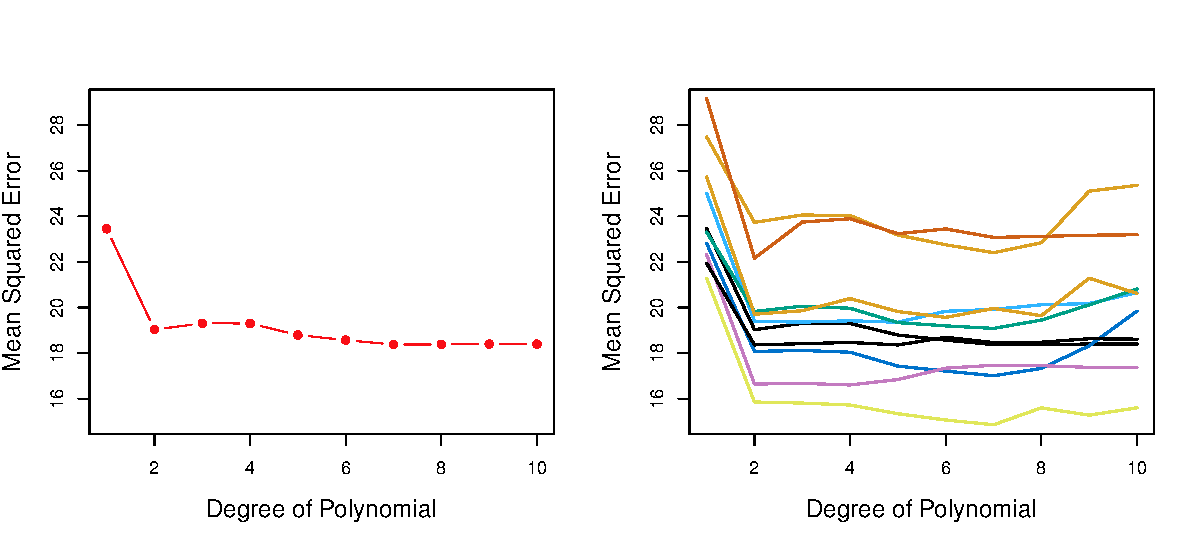
\includegraphics[width=0.7\textwidth]{5_2}
	\end{center}
	\vspace{-5mm}
	\begin{itemize}
		\item The \e{estimate} of the test error derived from the validation 
			set can be highly variable.
		\item The validation error tends to \e{overestimate} the test error rate
			due to the lower number of observations.
	\end{itemize}
	\bl{These issues are addressed by the various \e{cross-validation} methods.}
\end{frame}

\begin{frame}{Leave-One-Out Cross-Validation}
	\begin{center}
		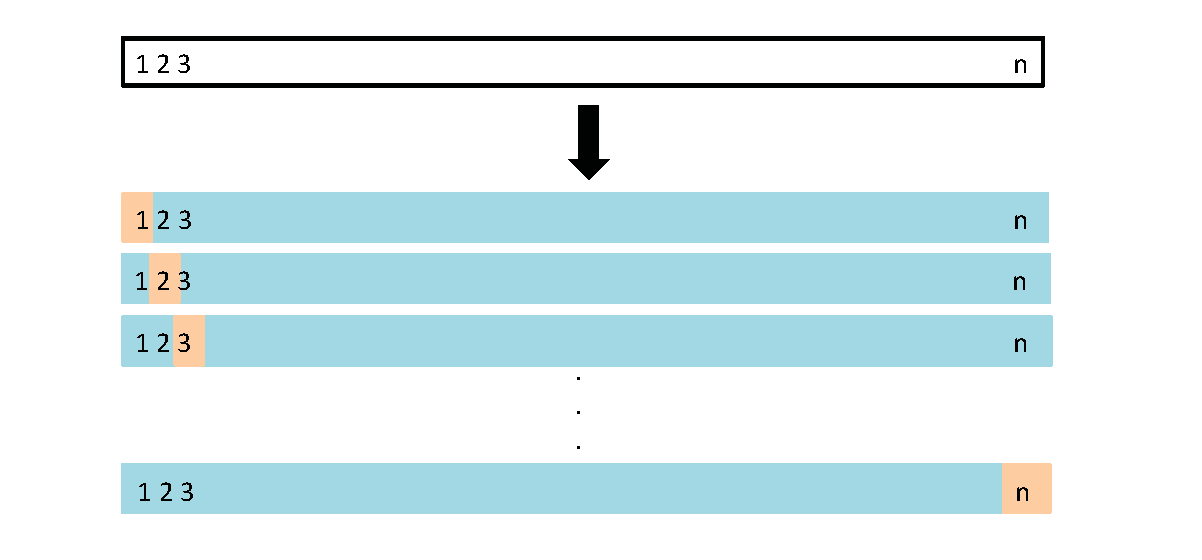
\includegraphics[width=0.8\textwidth]{5_3}
	\end{center}
	\bl{The LOOCV repeatedly uses \e{one} observation for validation.}
\end{frame}

\begin{frame}{Leave-One-Out Cross-Validation}
	\begin{itemize}
		\item The model fit is performed $n$ times.
		\item Where, as usual, $n$ is the number of training observations.
		\item We then average the MSE's from the $n$ fits:
			\[ 
				\text{CV}_{(n)} = 
				\frac{1}{n}\sum_{i=1}^{n} \text{MSE}_i
			\]
		\item That is, we sample the test set population and compute and estimate
			the test error.
	\end{itemize}
	\bl{The LOOCV has low bias but high variance.}
\end{frame}

\begin{frame}{$\bm{k}$-Fold Cross-Validation}
	\begin{center}
		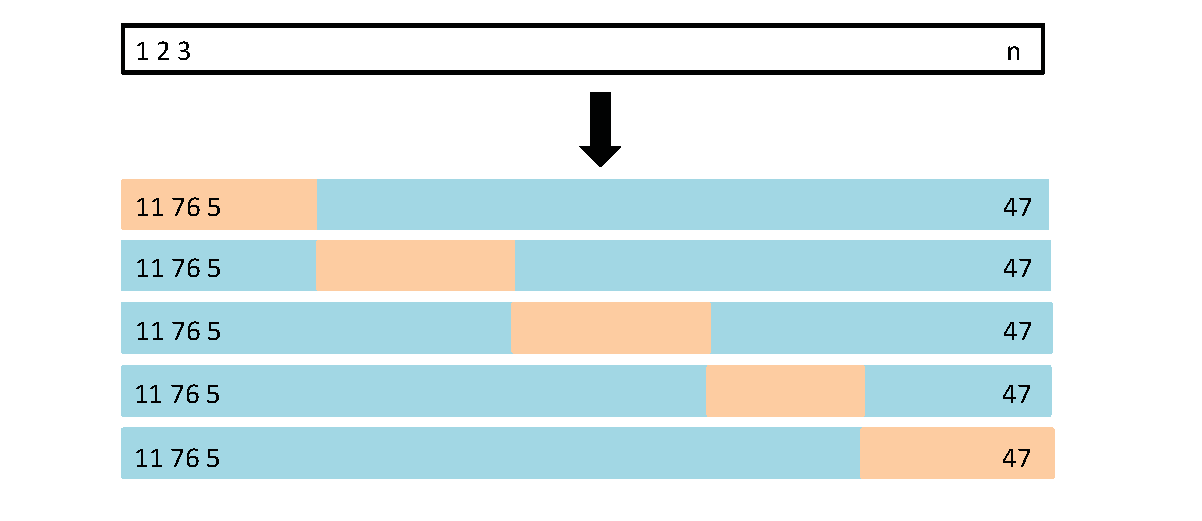
\includegraphics[width=0.8\textwidth]{5_5}
	\end{center}
	\bl{This approach repeatedly uses subsets of size $\bm{n/k}$ for validation.}
\end{frame}

\begin{frame}{$\bm{k}$-Fold Cross-Validation}
	\begin{itemize}
		\item Note that the training set is \e{randomly shuffled} before folding.
		\item The model fit is performed $k$ times.
		\item We then average the MSE's from the $k$ fits:
			\[ 
				\text{CV}_{(k)} = 
				\frac{1}{k}\sum_{i=1}^{k} \text{MSE}_i
			\]
		\item Again, we sample the test set population and compute and estimate
			the test error.
	\end{itemize}
	\bl{The bias-variance trade-off depends on the choice of $\bm{k}$.}
\end{frame}

\begin{frame}{Leave-One-Out versus $\bm{k}$-Fold Cross-Validation}
	\begin{center}
		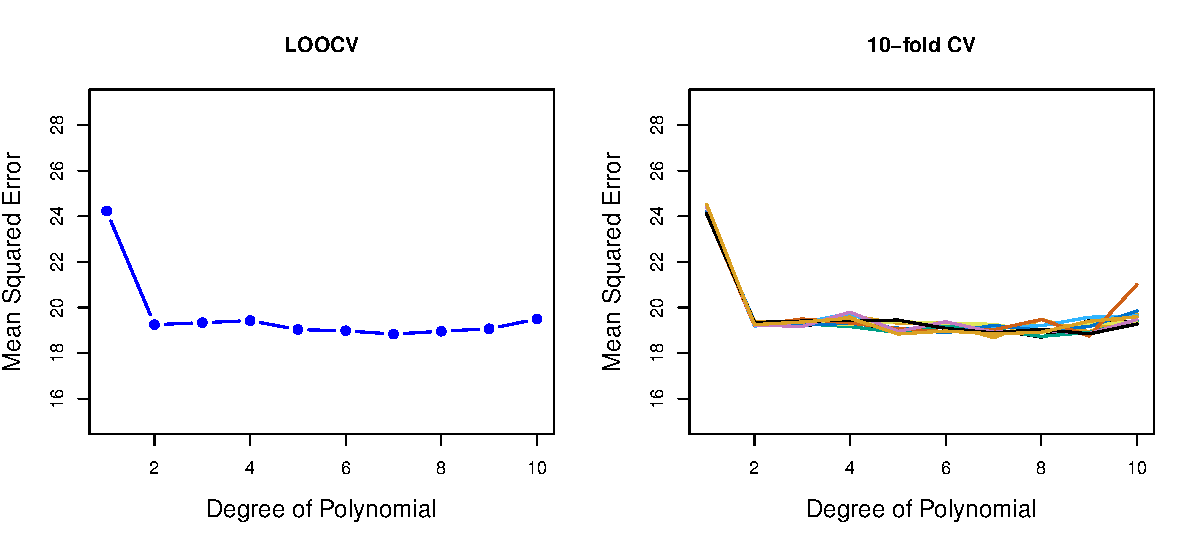
\includegraphics[width=0.8\textwidth]{5_4}

		LOOCV (left) and $10$-fold cross validation (right) on \dat{Auto}.
	\end{center}
	\bl{Values between 5 and 10 are typically good choices for for $\bm{k}$.}
\end{frame}

\begin{frame}{Leave-One-Out versus $\bm{k}$-Fold Cross-Validation}
	\begin{center}
		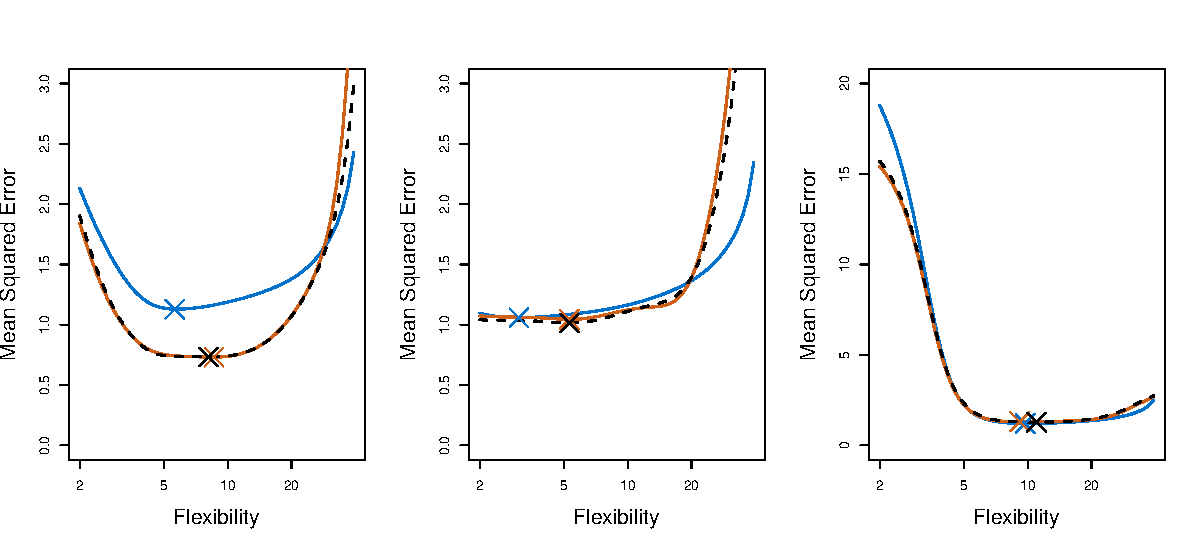
\includegraphics[width=0.8\textwidth]{5_6}

		LOOCV and $10$-fold cross validation on the simulated scenarios from lecture 2.
	\end{center}
	\bl{Close to the MSE minimum both methods have very similar results.}
\end{frame}

\begin{frame}{Cross-Validation for Classification}
	\begin{itemize}
		\item Cross-Validation also works in the classification setting.
		\item The misclassification rate takes the role of the MSE.
		\item For LOOCV the cross-validation error rate is
			\[ 
				\text{CV}_{(n)} = \frac{1}{n} \sum_{i=1}^n I(y_i\ne \hat{y}_1)
			\]
			with
			\[
				I(y_i\ne \hat{y}_i) =
				\begin{cases}
					1 & \text{if}\;\; y\ne \hat{y}_i\\
					0 & \text{if}\;\; y = \hat{y}_i\\
				\end{cases}
			\]
	\end{itemize}
	\bl{We can evaluate classification models just like regression models.}
\end{frame}

\begin{frame}{Cross-Validation for Classification}
	\begin{columns}
		\begin{column}{0.5\textwidth}
			\begin{itemize}
				\item The figures show four different polynomial
					logistic regression models.
				\item Non-linear terms can be added to the logistic model just like
					in linear regression.
				\item For example, the quadratic (Degree=2) model is
					\begin{align*}
						\log\left(\frac{p}{1-p}\right) & =
						&\beta_0&+ \beta_1 X_1 + \beta_2 X_1^2\\
						&\phantom{=} &\phantom{\beta_0}&+ \beta_3 X_2 + \beta_4 X_2^2\\
					\end{align*}
			\end{itemize}
			\bl{A degree > 3 doesn't help much anymore.}
		\end{column}
		\begin{column}{0.5\textwidth}
			\vspace{-10mm}
			\begin{center}
				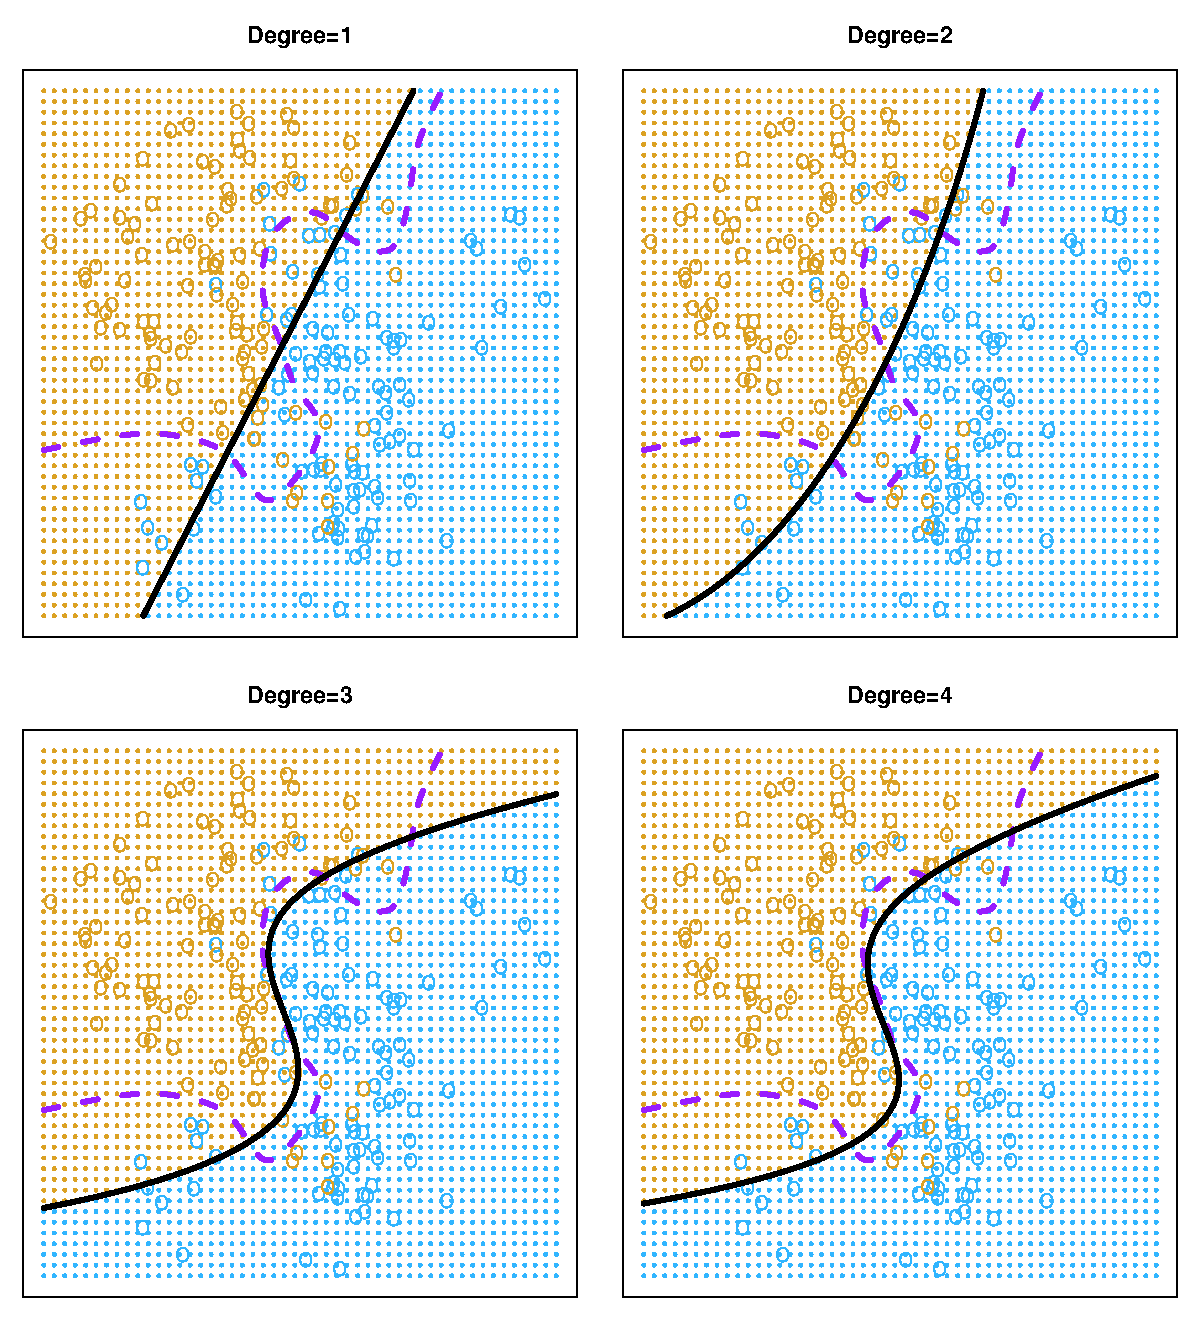
\includegraphics[width=0.95\textwidth]{5_7}
			\end{center}
		\end{column}
	\end{columns}
\end{frame}

\begin{frame}{Cross-Validation for Classification}
	\vspace{-10mm}
	\begin{center}
		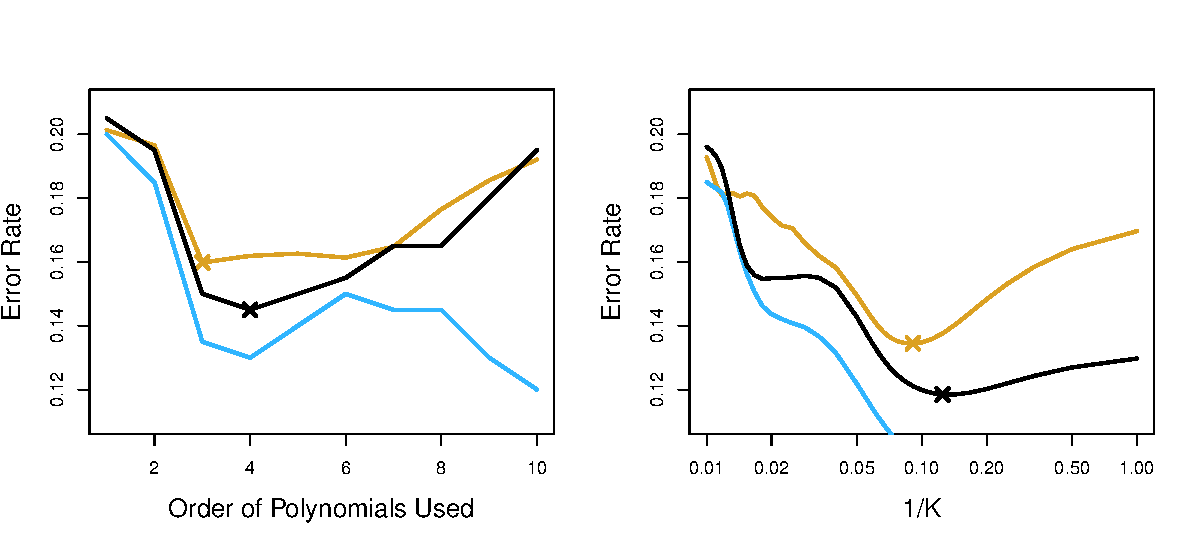
\includegraphics[width=0.8\textwidth]{5_8}
	\end{center}
	\vspace{-7mm}
	\begin{itemize}
		\item The figures show various polynomial models (left) and an KNN classifier (right).
		\item The test error ({\orange orange}), training error ({\blue blue}) and
			cross-validation error ({\color{black} black}) are shown.
		\item The $K$ in the right plot denotes the neighbours in KNN.
	\end{itemize}
	\bl{The test error is obtained from a simulated test sample.}
\end{frame}

\begin{frame}{The Bootstrap Method}
	\begin{itemize}
		\item \e{Bootstrap} is widely applicable method to assess model uncertainties.
		\item We demonstrate it on a simulated toy example.
		\item Suppose we have some money we want to invest.
		\item We would like to invest a fraction $\alpha$ in an asset with return $X$ 
			and the rest, $1 - \alpha$,\\ in an asset with return $Y$ such that the risk is minimised.
		\item The risk is associated with the variance of the total return:
			\[ \text{Var}\left(\alpha X + (1 - \alpha) Y \right) \]
			which is minimal when
			\[
				\alpha = 
				\frac{\sigma^2_Y - \sigma_{XY}}
				{\sigma^2_X + \sigma^2_Y - 2\sigma_{XY}}
			\]
	\end{itemize}
	\bl{In practice, we have to estimate $\bm{\sigma^2_X}$, $\bm{\sigma^2_Y}$
	and $\bm{\sigma_{XY}}$ from the training data.}
\end{frame}

\begin{frame}{The Bootstrap Method}
	\begin{itemize}
		\item In the toy simulation the true values are $\sigma^2_X = 1$,
			$\sigma^2_Y = 1.25$ and $\sigma_{XY} = 0.5$.
		\item The $\alpha$ with minimal risk  is then $\alpha = 0.6$.
		\item We simulate 1000 independent samples with 100 observations each to obtain
			\[
				\hat{\alpha} = \overline{\alpha} = \frac{1}{1000}
				\sum_{r=1}^{1000} \hat{\alpha}_r = 0.5996
			\]
			and the error estimate
			\[
				\widehat{\text{SE}}(\overline{\alpha}) =
				\sqrt{
					\frac{1}{1000 - 1}
					\sum_{r=1}^{1000} \left( \hat{\alpha}_r - \overline{\alpha}\right)
				}
				= 0.083
			\]
	\end{itemize}
	\bl{In practice, we don't have a large number of independent samples.}
\end{frame}

\begin{frame}{The Bootstrap Method}
	\begin{columns}
		\begin{column}{0.5\textwidth}
			\begin{itemize}
				\item In the absence of independent test samples we need
					a different solution.
				\item The \e{bootstrap} method creates test samples by
					repeatedly sampling from the training data.
				\item The sampling is done with \e{replacement}.
				\item That is, an observation can appear more than once
					in each sample.
				\item Sampling $B$ times we obtain
					{\footnotesize
					\[
						\widehat{\text{SE}}(\hat{\alpha}) =
						\sqrt{
							\frac{1}{B -1}
							\sum_{r=1}^B
							\left(
							\hat{\alpha}^{*r} -
								\frac{1}{B}
								\sum_{r' = 1}^B \hat{\alpha}^{*r'}
							\right)^2
						}
					\]}
			\end{itemize}
		\end{column}
		\begin{column}{0.5\textwidth}
			\begin{center}
				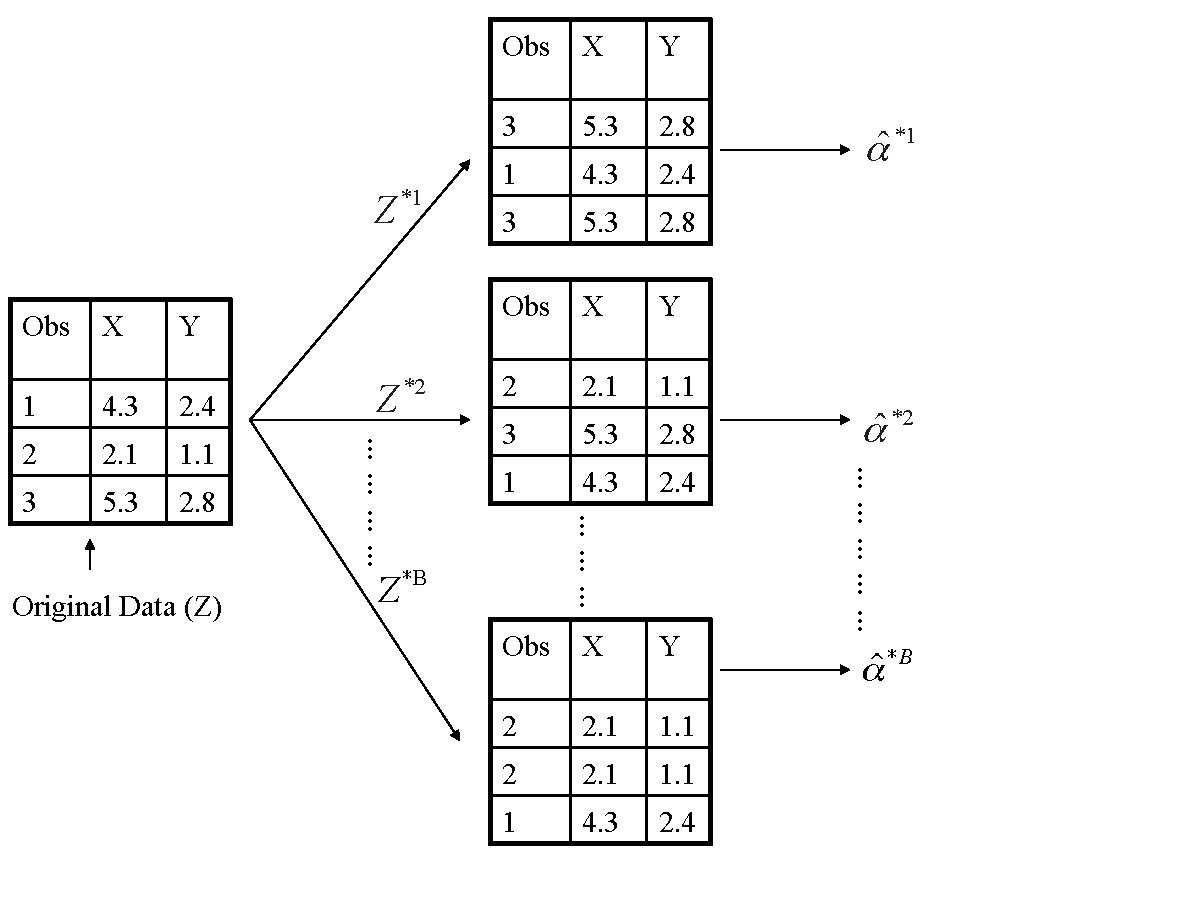
\includegraphics[width=1.0\textwidth]{5_11}
			\end{center}
		\end{column}
	\end{columns}
	\bl{In practice, $\bm{B}$ needs to be sufficiently large, $\bm{\mathcal{O}(1000)}$.} 
\end{frame}

\begin{frame}{The Bootstrap Method}
	\begin{center}
		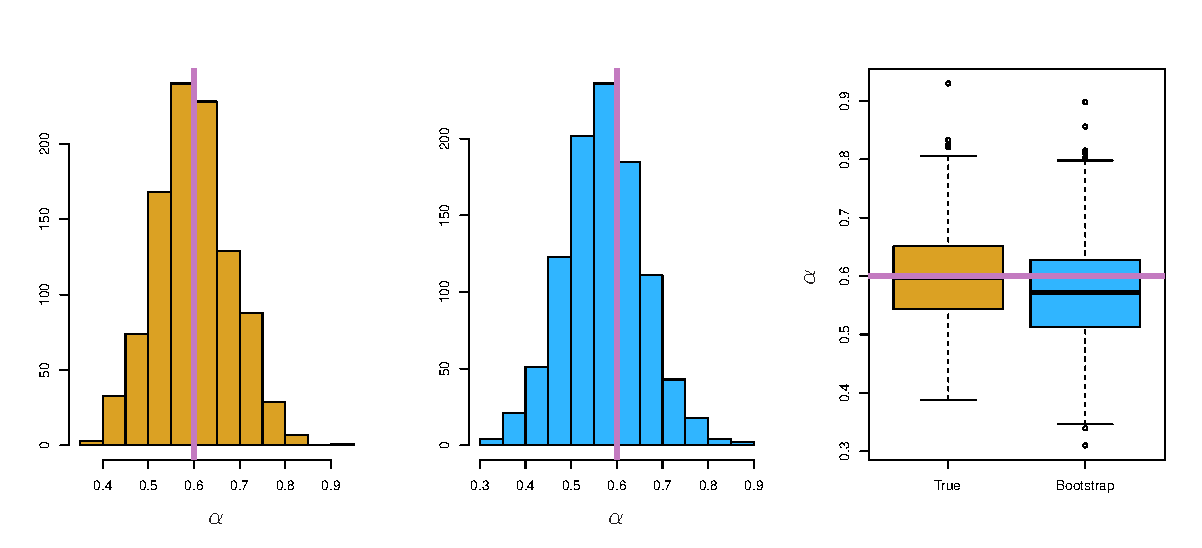
\includegraphics[width=0.9\textwidth]{5_10}
	\end{center}
	\bl{We can see that the bootstrap method does very well.}
\end{frame}
\end{document}
